% BCS-BEC Crossover 的平均场描述
% 玻色爱因斯坦|凝聚态|平均场

仍然沿用BCS的Hamiltonian,在动量空间里面,
\begin{equation}
H-\mu N = \sum_{{\bvec k},\sigma}(\epsilon_{\bvec k}-\mu)a\Her_{{\bvec k},\sigma}a_{\bvec k, \bvec \sigma}+\frac{1}{V}\sum_{\bvec k,  \bvec k'}U_{\bvec k, \bvec k'}a\Her_{\bvec k\uparrow}a\Her_{-\bvec k\downarrow}a_{-\bvec k\downarrow}a_{\bvec k\uparrow}
\end{equation}

假设不是一个微扰的情况下,也可以用 $|\Psi\rangle = \prod_{\bvec k}(u_{\bvec k}+v_{\bvec k}a\Her_{\bvec k\uparrow}a\Her_{-\bvec k\downarrow})|0\rangle$ 来描述基态. 仍然定义平均场参数 $\Delta = \langle a_{-\bvec k\downarrow},a_{\bvec k\uparrow}\rangle$. 不同的是,研究冷原子问题的时候,并不是只有在费米面附近才有 $U$,而是一个队任意动量都可以的情况. 重复同样的Bogoliubov变换,我们能够解出来 $u_{\bvec k}^2, v_{\bvec k}^2 = 1/2(1\pm\epsilon_{\bvec k}/E_{\bvec k})$,其中元激发的能级关系$E_{\bvec k}=\sqrt{(\epsilon_{\bvec k}-\mu)^2+|\Delta|^2}$. 利用自洽方程,我们得到
\begin{equation}
-\frac{1}{U} = \frac{1}{V}\sum_{\bvec k}\frac{1}{2E_{\bvec k}}
\end{equation}
而我们知道,“两个原子间的相互作用\upref{TwoAtF}” 中\autoref{TwoAtF_eq38} 给出了
\begin{equation}
\frac{ma_s}{4\pi\hbar^2} = \frac{1}{g} + \frac{1}{V}\sum_{\bvec k}\frac{1}{\hbar^2{\bvec k}^2/m} = \frac{1}{V}\sum_{\bvec k}\left(\frac{1}{2\epsilon_{\bvec k}} - \frac{1}{2E_{\bvec k}}\right)
\end{equation}
定义无量纲参数来简化问题:
\begin{equation}
x^2 = \frac{\hbar^2{\bvec k}^2}{2m}\frac{1}{\Delta},\quad x_0 = \frac{\mu}{\Delta},\quad \epsilon_x = x^2-x_0 = \frac{\epsilon_{\bvec k}-\mu}{\Delta},\quad E_x = \sqrt{1+\epsilon_x^2} = \frac{E_{\bvec k}}{\Delta}
\end{equation}
把求和化为积分,也就是 $\frac{1}{V}\sum_{\bvec k}\to\int_0^\infty \text{d}^3{\bvec k}/(2\pi)^3$,利用求对称性,我们很容易转写一些式子:
\begin{equation}
\begin{split}
-\frac{m\Delta}{4\pi\hbar^2 a_s} &=\frac{1}{V}\sum_{\bvec k}\left(\frac{\Delta}{2E_{\bvec k}} - \frac{\Delta}{2\epsilon_{\bvec k}}\right)\\
-\frac{m\Delta}{4\pi\hbar^2 a_s} &=\int_0^\infty\frac{\text{d}^3{\bvec k}}{(2\pi)^3}\left(\frac{1}{2E_x} - \frac{1}{2x^2}\right) \\
&=\int_0^\infty\frac{\text{d}k\cdot 4\pi k^2}{(2\pi)^3}\left(\frac{1}{2E_x} - \frac{1}{2x^2}\right)\\
-\frac{1}{a_s} &= \frac{2}{\pi\Delta}\frac{\hbar^2}{m}\int_0^\infty\text{d}k\cdot k^2\left(\frac{1}{2E_x} - \frac{1}{2x^2}\right)\\
k^2 &= \frac{mx^2}{\hbar^2}\\
-\frac{1}{a_s} &= \frac{2}{\pi}\sqrt{\frac{2m\Delta}{\hbar^2}}\int_0^\infty \text{d}x\cdot x^2\left(\frac{1}{E_x}-\frac{1}{x^2}\right)
\end{split}
\end{equation}
可以看出来,右边的积分纯粹只是 $x_0$ 的函数,可以定义
\begin{equation}
I_1(x_0) = \int_0^\infty \text{d}x\cdot x^2\left(\frac{1}{E_x}-\frac{1}{x^2}\right)
\end{equation}

而另一方面,我们可以根据热力学定律知道平均粒子数 $N=-\partial\Omega/\partial\mu$ 得到
\begin{equation}
N = \sum_{\bvec k}\left(1-\frac{\epsilon_{\bvec k}-\mu}{E_{\bvec k}}\right)
\end{equation}
而这个 $N$ 是要满足我们的要求的,也就是说 $n=N/V=k_F^3/(3\pi^2)$. 我们当然也可以用类似的无量纲参数来处理:
\begin{equation}
\begin{split}
n &= \frac{1}{V}\sum_{\bvec k}\left(1-\frac{\epsilon_{\bvec k}-\mu}{E_{\bvec k}}\right)\\
&=\frac{1}{V}\sum_{\bvec k}\left(1-\frac{\epsilon_x{\Delta}}{E_x{\Delta}}\right)\\ % 未完成, 这里分子分母两个 delta 是被 \cancel 掉的, 然而这个命令编译不出来
&=\int_0^\infty\frac{\text{d}k \cdot 4\pi k^2}{(2\pi)^3}\left(1-\frac{\epsilon_x}{E_x}\right)\\
&=\frac{1}{2\pi^2}\frac{2m\Delta}{\hbar^2}\sqrt{\frac{2m\Delta}{\hbar^2}}\int_0^\infty\text{d}x\cdot x^2\left(1-\frac{\epsilon_x}{E_x}\right)\\
&=\frac{1}{2\pi^2}\left(\frac{2m\Delta}{\hbar^2}\right)^{3/2}I_2(x_0)
\end{split}
\end{equation}
其中
\begin{equation}
I_2(x_0)=\int_0^\infty \text{d}x\cdot x^2\left(1-\frac{\epsilon_x}{E_x}\right)
\end{equation}

于是我们得到了两个方程(代替原本的自洽方程来给我们关于系统的信息)
\begin{equation}
\begin{cases}
\dfrac{\Delta}{E_F} = \left(\dfrac{2}{3I_2(x_0)}\right)^{2/3}\\
\ \\
\dfrac{1}{k_Fa_s} = -\dfrac{2}{\pi}\left(\dfrac{2}{3I_2(x_0)}\right)^{1/3}I_1(x_0)
\end{cases}
\end{equation}

\begin{figure}[ht]
\centering
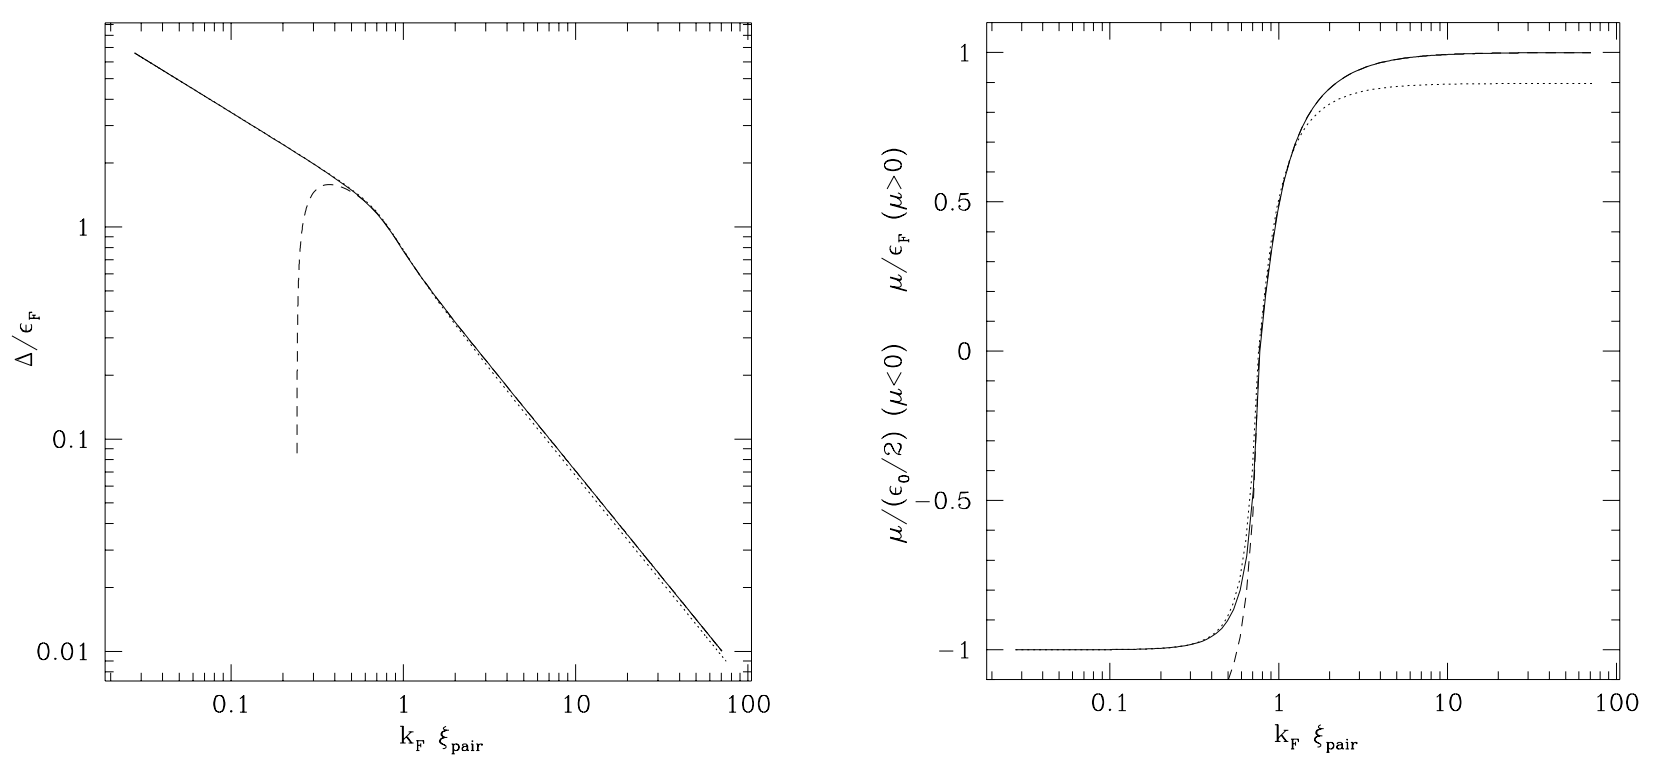
\includegraphics[width=15cm]{./figures/BCSBEC_1.png}
\caption{左:$\Delta/E_F$ vs $k_F\xi_{\text{pair}}$,右:$\mu/E_F(\mu>0), \mu/(\epsilon_0/2)(\mu<0)$,区分两种情况是因为在Bose情况下没有费米能的定义,$\epsilon_0\equiv1/(ma_s^2)$} \label{BCSBEC_fig1}
\end{figure}

但是,对于 $I_1, I_2$ 的渐进行为并不好分析,我们定义更多的积分
\begin{align}
I_3(x_0) &=\int_0^\infty\text{d}x\frac{x^4\epsilon_x}{E_x^6}\\
I_4(x_0) &=\int_0^\infty\text{d}x\frac{x^2}{E_x^2}\\
I_5(x_0) &=\int_0^\infty\text{d}x\frac{x^2}{E_x^3}\\
I_6(x_0) &=\int_0^\infty\text{d}x\frac{x^2\epsilon_x}{E_x^3}
\end{align}

可以知道, $I_1=(2x_0I_6-I_5),I_2 = \frac{2}{3}(x_0I_5+I_6)$. 而 $I_3,I_4$ 是很好计算的. 如果定义
\begin{equation}
x_1^2=\frac{x_0+\sqrt{1+x_0^2}}{2}
\end{equation}
就可以算出
\begin{align}
I_3&=\frac{\pi}{16}\frac{x_1(1+x_1^4)}{(1+x_0^2)^{1/2}}\\
I_4&=\frac{\pi}{2}x_1
\end{align}

平均场下可以计算费米子对的特征距离
\begin{equation}
\xi_{\text{pair}}^2 = \frac{1}{m^2}\frac{\int_0^\infty\text{d}k(k^4(\epsilon_{\bvec k}-\mu)^2/E_{\bvec k}^6)}{\int_0^\infty\text{d}k(k^2/E_{\bvec k}^2)} = \frac{2}{m\Delta}\frac{I_3}{I_4}
\end{equation}

还有一些其他的参数信息
\begin{align}
\frac{\Delta}{E_F} &= \left(\frac{1}{x_0I_5+I_6}\right)^{2/3}\\
\frac{\mu}{E_F} &= x_0\frac{\Delta}{E_F} \\
\frac{1}{k_Fa_s} &= -\frac{4}{\pi}\frac{x_0I_6-I_5}{(x_0I_5+I_6)^{1/3}}\\
k_F\xi_{\text{pair}} &= \sqrt{\frac{1+x_1^4}{2}}\frac{(x_0I_5+I_6)^{1/3}}{(1+x_0^2)^{1/4}}
\end{align}

现在仔细分析一下渐进行为:

\begin{itemize}
\item $x_0\to\infty$,此时 $\mu\to E_F$, $I_5\sim\sqrt{x_0}$, $I_6\sim\ln x_0/(2\sqrt{x_0})$,我们的 $1/k_Fa_s\to(2/\pi)\ln x_0$, $a_s\to0^+$,表现为微弱的吸引力,就是BCS态的情况. 此时 $k_F\xi_{\text{pair}}\to x_0/\sqrt2$.
\item $x_0\to-\infty$, $I_5\sim\pi/(16|x_0|^{3/2}), I_6\sim\pi/(4|x_0|^{1/2})$. 此时 $\Delta\to\infty, \mu\to-\infty, a_s\to0^+,k_F\xi_{\text{pair}}\to0^+$. 表现为强吸引力($\Delta$),就是BEC极限.
\end{itemize}

可以用 $k_f\xi_{\text{pair}}$ 作为参数反解很多信息,如\autoref{BCSBEC_fig1}.


